\documentclass[pdflatex,compress,mathserif]{beamer}

%\usetheme[dark,framenumber,totalframenumber]{ElektroITK}
\usetheme[darktitle,framenumber,totalframenumber]{ElektroITK}

\usepackage[utf8]{inputenc}
\usepackage[T1]{fontenc}
\usepackage{lmodern}
\usepackage[bahasai]{babel}
\usepackage{amsmath}
\usepackage{amsfonts}
\usepackage{amssymb}
\usepackage{graphicx}
\usepackage{multicol}
\usepackage{lipsum}
\usepackage{framed}
\usefonttheme[onlymath]{serif}

\newcommand*{\Scale}[2][4]{\scalebox{#1}{$#2$}}%

\setbeamertemplate{caption}[numbered]

\title{PENGOLAHAN SINYAL DIGITAL}
\subtitle{Proses Sampling}

\author{Mifta Nur Farid}

\begin{document}

\maketitle

\section{Sampling}

\begin{frame}{Diagram blok pengolahan\\sinyal digital}
    \begin{figure}
        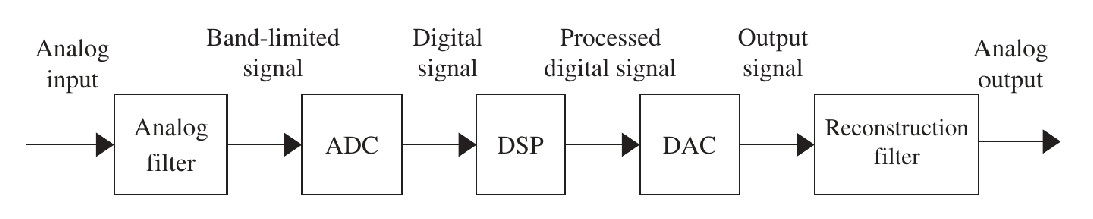
\includegraphics[width=\linewidth]{./img/img01.png}
    \end{figure}
\end{frame}

\begin{frame}{Proses sampling dalam domain\\waktu}
    \begin{itemize}
        \item Sinyal waktu kontinyu memiliki titik yang tak berhingga
        \item Tidak mungkin mendigitalkan titik yang tak berhingga karena membutuhkan banyak memory dalam komputasinya
        \item Solusinya $\rightarrow$ sampling $\rightarrow$ T = sampling interval atau sampling period (detik)
        \begin{figure}
            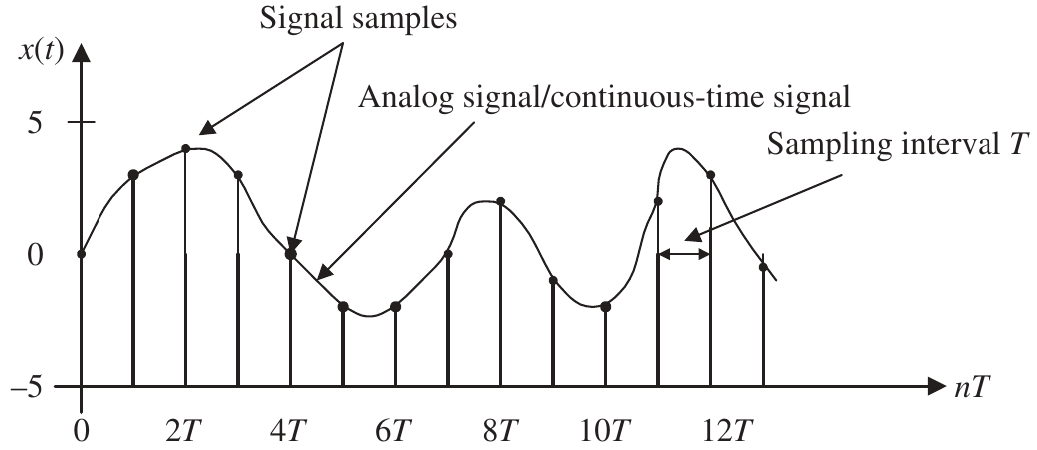
\includegraphics[width=0.9\linewidth]{./img/img02.png}
        \end{figure}
    \end{itemize}
\end{frame}

\begin{frame}{Sample-and-hold tegangan analog\\untuk ADC}
    \begin{itemize}
        \item Setiap sample mempertahankan nilai tegangannya selama interval $T$ $\rightarrow$ memberikan cukup waktu untuk ADC mengubahnya
        \item Metode sampling: \textbf{Sample-and-Hold}
        \begin{figure}
            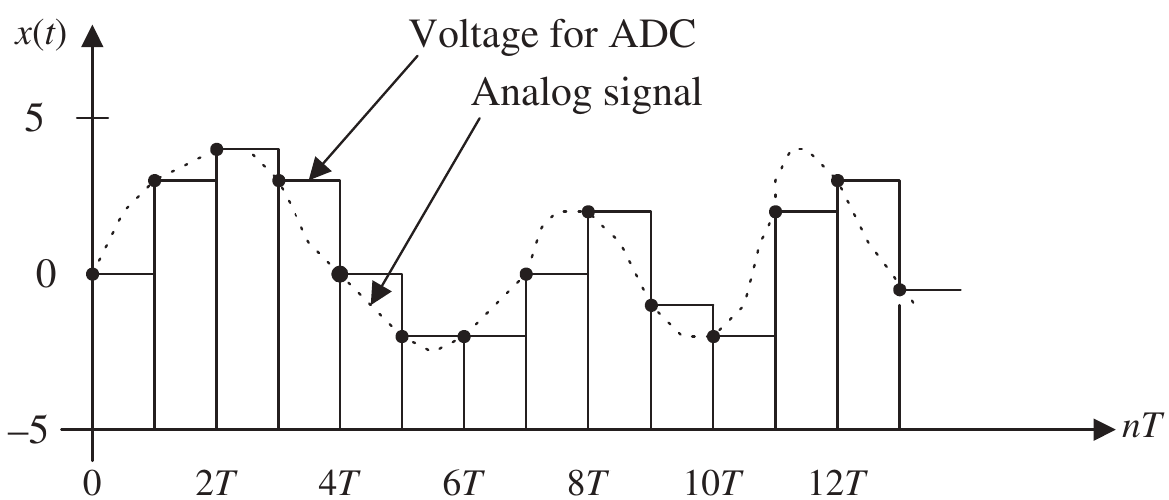
\includegraphics[width=0.9\linewidth]{./img/img03.png}
        \end{figure}
    \end{itemize}
\end{frame}

\begin{frame}{Sampling rate}
    \begin{itemize}
        \item Untuk setiap sampling interval $T$ yang diberikan, sampling rate $f_s$ adalah
        \begin{equation}
            f_s = \frac{1}{T} \text{ samples per second (Hz)}
        \end{equation}
        \item Contoh: jika sampling period, $T$ = 125 $\mu s$, maka sampling rate adalah $$ f_s = \frac{1}{125 \mu s} = 8000 \text{ Hz} $$
    \end{itemize}
\end{frame}

\begin{frame}{Teorema Sampling}
    \begin{itemize}
        \item Berapa minimum sampling rate yang dibutuhkan?
    \end{itemize}    
\end{frame}

\begin{frame}{Teorema Sampling}
    \begin{itemize}
        \item Sinyal analog 40 Hz, sampling period T = 0.01 detik, sehingga sampling rate $f_s = \frac{1}{T} = \frac{1}{0.01} = 100$ Hz
        \item Sinyal sampled masih terlihat sama dengan sinyal analog
        \begin{figure}
            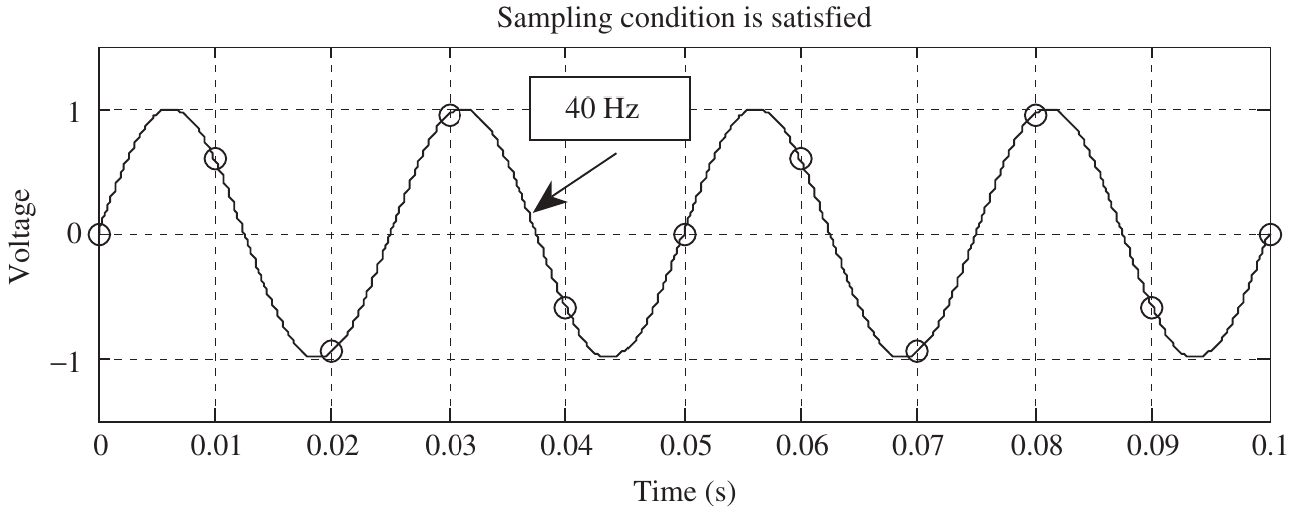
\includegraphics[width=\linewidth]{./img/img04.png}
        \end{figure}
    \end{itemize}
\end{frame}

\begin{frame}{Teorema Sampling}
    \begin{itemize}
        \item Sinyal analog 90 Hz, sampling period T = 0.01 detik, sehingga sampling rate $f_s = \frac{1}{T} = \frac{1}{0.01} = 100$ Hz
        \item Sinyal sampled terlihat memiliki frekuensi 10 Hz.
        \begin{figure}
            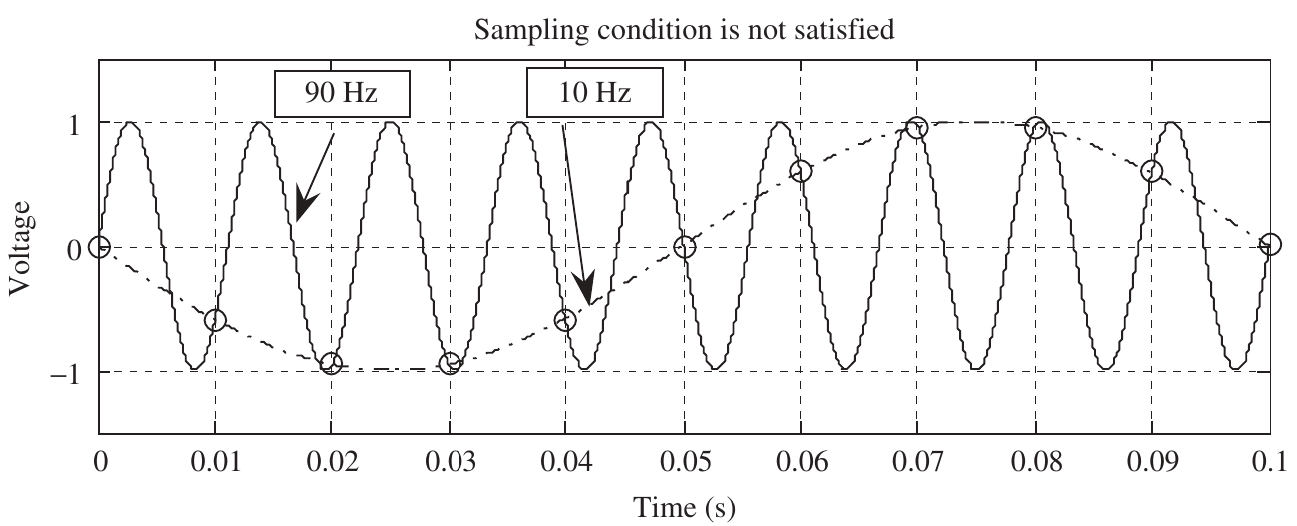
\includegraphics[width=\linewidth]{./img/img05.png}
        \end{figure}
    \end{itemize}
\end{frame}

\begin{frame}{Teorema Sampling}
    \begin{itemize}
        \item Sehingga ada nilai minimum dari sampling rate.
        \item Sinyal sampled akan memiliki frekuensi yang sama selama sampling rate-nya minimal 2 kali daripada komponen frekuensi tertinggi dari sinyal analognya

        \begin{equation}
            f_s \geq 2 f_\text{max}
        \end{equation}

        $f_\text{max}$ adalah komponen frekuensi tertinggi dari sinyal analog
        \item Sehingga dari ilustrasi sebelumnya, sampling rate minimal untuk sinyal analog 90 Hz adalah 2$\times$90 Hz = 180 Hz
    \end{itemize}
\end{frame}

\begin{frame}{Teorema Sampling}
    \begin{itemize}
        \item Berapa sampling rate minimum untuk sinyal analog berikut ini?
        \begin{multicols}{2}
            \begin{enumerate}
                \item[a.] 500 Hz
                \item[b.] 1000 Hz
                \columnbreak
                \item[c.] 1500 Hz
                \item[d.] 2000 Hz
            \end{enumerate}
        \end{multicols}
        \begin{figure}
            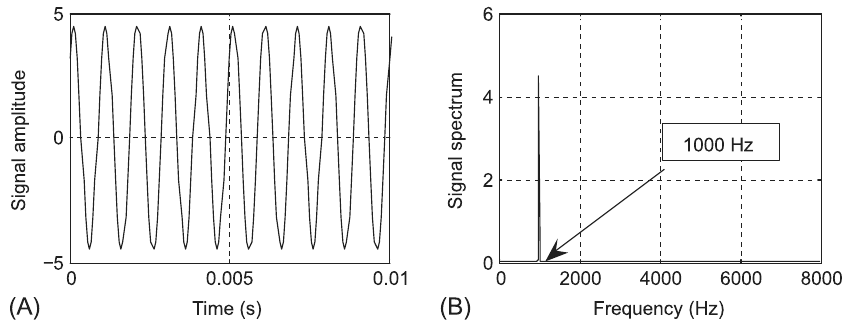
\includegraphics[width=\linewidth]{./img/img06}
        \end{figure}
    \end{itemize}
\end{frame}

\begin{frame}{Teorema Sampling}
    \begin{itemize}
        \item Berapa sampling rate minimum untuk sinyal analog berikut ini?
        \begin{multicols}{2}
            \begin{enumerate}
                \item[a.] 2000 Hz
                \item[b.] 4000 Hz
                \columnbreak
                \item[c.] 6000 Hz
                \item[d.] 8000 Hz
            \end{enumerate}
        \end{multicols}
        \begin{figure}
            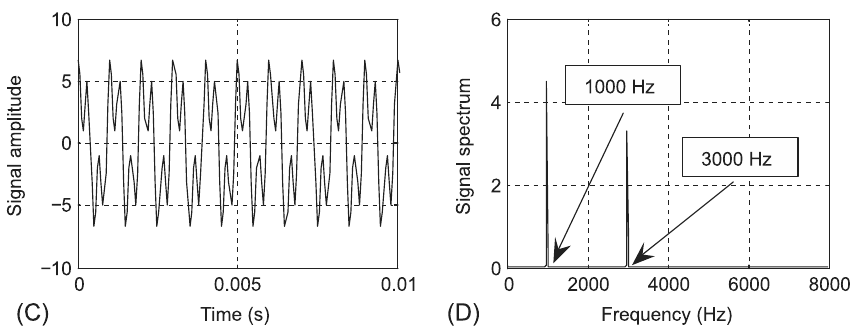
\includegraphics[width=\linewidth]{./img/img07}
        \end{figure}
    \end{itemize}
\end{frame}

\begin{frame}{Teorema Sampling}
    \begin{figure}
        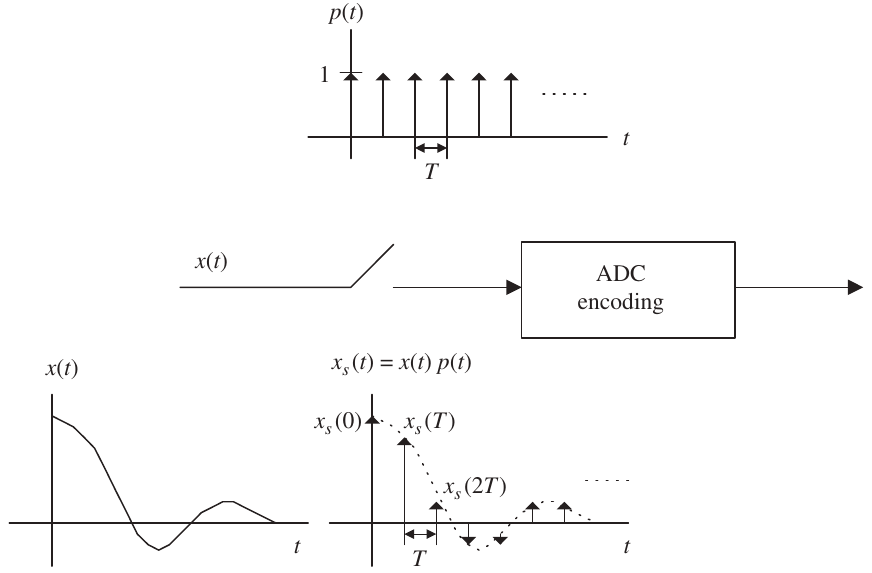
\includegraphics[width=0.9\linewidth]{./img/img08}
    \end{figure}
\end{frame}

\begin{frame}{Teorema Sampling}
    \begin{itemize}
        \item Proses sampling
        \begin{equation}
            x_s(t) = x(t) p(t)
            \label{eq:xs}
        \end{equation}
        yang mana $p(t)$ adalah pulse train dengan period $T = \frac{1}{f_s}$
        \item Pulse train:
        \begin{equation}
            p(t) = \sum_{n = - \infty}^\infty \delta(t - nT)
        \end{equation}
    \end{itemize}
\end{frame}

\begin{frame}{Teorema Sampling}
    \begin{itemize}
        \item Dengan frekuensi dasar, $\omega_0 = 2\pi/T = 2\pi f_s$ rad/s, $p(t)$ dapat direpresentasikan dalam bentuk deret Fourier
        \begin{equation}
            p(t) = \sum_{k = - \infty}^\infty a_k e^{jk\omega_0t}
            \label{eq:pt_deret}
        \end{equation}
        yang mana $a_k$ adalah koef. Fourier yang dapat ditentukan oleh
        \begin{equation}
            a_k = \frac{1}{T} \int_{-\infty}^{\infty} \delta(t)e^{-jk\omega_0t}dt = \frac{1}{T}
            \label{eq:keof.Fourier}
        \end{equation}
    \end{itemize}
\end{frame}

\begin{frame}{Teorema Sampling}
    \begin{itemize}
        \item Substitusikan Pers. (\ref{eq:keof.Fourier}) ke Pers. (\ref{eq:pt_deret}), didapatkan
        \begin{equation}
            p(t) = \sum_{k = -\infty}^{\infty} \frac{1}{T} e^{jk\omega_0t}
            \label{eq:pt_new}
        \end{equation}
        \item Substitusikan Pers. (\ref{eq:pt_new}) ke Pers. (\ref{eq:xs}), didapatkan
        \begin{equation}
            x_s(t) = \sum_{k = -\infty}^{\infty} \frac{1}{T} x(t) e^{jk\omega_0t}
            \label{eq:xs_new}
        \end{equation}
    \end{itemize}
\end{frame}

\begin{frame}{Teorema Sampling}
    \begin{itemize}
        \item Transformasi Fourier dari Pers. (\ref{eq:xs_new}):
        \begin{align}
            X_s(f) &= \text{FT} \left\{ \sum_{k = -\infty}^{\infty} \frac{1}{T} x(t) e^{jk\omega_0t} \right\} \\
            &= \sum_{k = -\infty}^{\infty} \frac{1}{T} \text{ FT} \left\{ x(t) e^{jk\omega_0t} \right\} \\
            &= \sum_{k = -\infty}^{\infty} \frac{1}{T} \int_{-\infty}^{\infty} \left\{ x(t) e^{jk\omega_0t} \right\}e^{-j\omega t} dt\\
            &= \sum_{k = -\infty}^{\infty} \frac{1}{T} \int_{-\infty}^{\infty} x(t) e^{-j(\omega-k\omega_0) t} dt \\
            X_s(f) &= \sum_{k = -\infty}^{\infty} \frac{1}{T} \int_{-\infty}^{\infty} x(t) e^{-j2\pi(f-kf_s) t} dt
            \label{eq:Xsf}
        \end{align}
    \end{itemize}
\end{frame}

\begin{frame}{Teorema Sampling}
    \begin{itemize}
        \item Berdasarkan definisi dari Transformasi Fourier, kita tahu bahwa
        \begin{equation}
            X(f) = \sum_{k = -\infty}^{\infty} \frac{1}{T} \int_{-\infty}^{\infty} x(t) e^{-j2\pi ft} dt
            \label{eq:Xf}
        \end{equation}
        \item Kita dapatkan hubungan antara Pers. (\ref{eq:Xf}) dan Pers. (\ref{eq:Xsf})
        \begin{equation}
            X_s(f) = \frac{1}{T} \sum_{k = -\infty}^{\infty} X(f - kf_s)
            \label{eq:Xsf_and_Xf}
        \end{equation}
        yang mana $X(f)$ adalah spectrum sinyal asli sedangkan $X_s(f)$ spectrum sinyal sampled yang terdiri dari spectrum sinyal asli $X(f)$ dan kembarannya $X(f\pm kf_s)$
    \end{itemize}
\end{frame}

\begin{frame}{Teorema Sampling}
    \begin{itemize}
        \item Kita lanjutkan Pers. (\ref{eq:Xsf_and_Xf}):
        \begin{equation}
            X_s(f) = \cdots + \frac{1}{T}X(f+f_s) + \frac{1}{T}X(f) + \frac{1}{T}X(f-f_s) + \cdots
            \label{eq:deret_Xsf_and_Xf}
        \end{equation}
        \item spectrum sinyal sample, $X_s(f)$, merupakan penjumlahan dari scaled spectrum sinyal asli, $ \frac{1}{T} X(f) $, dan scaled spectrum kembarannya, $ \frac{1}{T} X(f \pm f_s) $.
        \item Pers. (\ref{eq:deret_Xsf_and_Xf}) memiliki kemungkinan 3 grafik berdasarkan nilai sampling rate-nya ($f_s$)
    \end{itemize}
\end{frame}

\begin{frame}{Teorema Sampling}
    \begin{itemize}
        \item Kondisi 1: spectrum sinyal sample terpisah dengan kembarannya
        \begin{figure}
            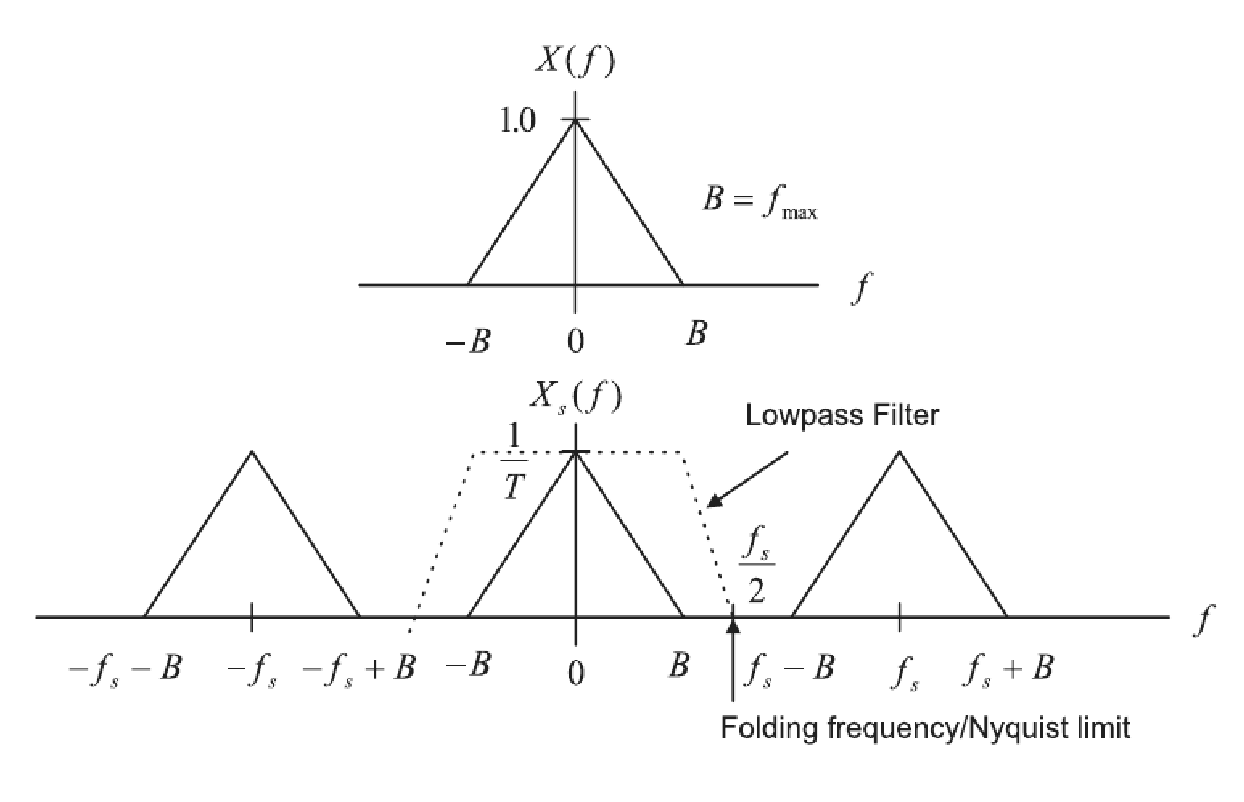
\includegraphics[width=0.9\linewidth]{./img/img09}
            \label{img:09}
        \end{figure}
    \end{itemize}
\end{frame}

\begin{frame}{Teorema Sampling}
    \begin{itemize}
        \item Kondisi 2: spectrum sinyal sample terhubung dengan kembarannya
        \begin{figure}
            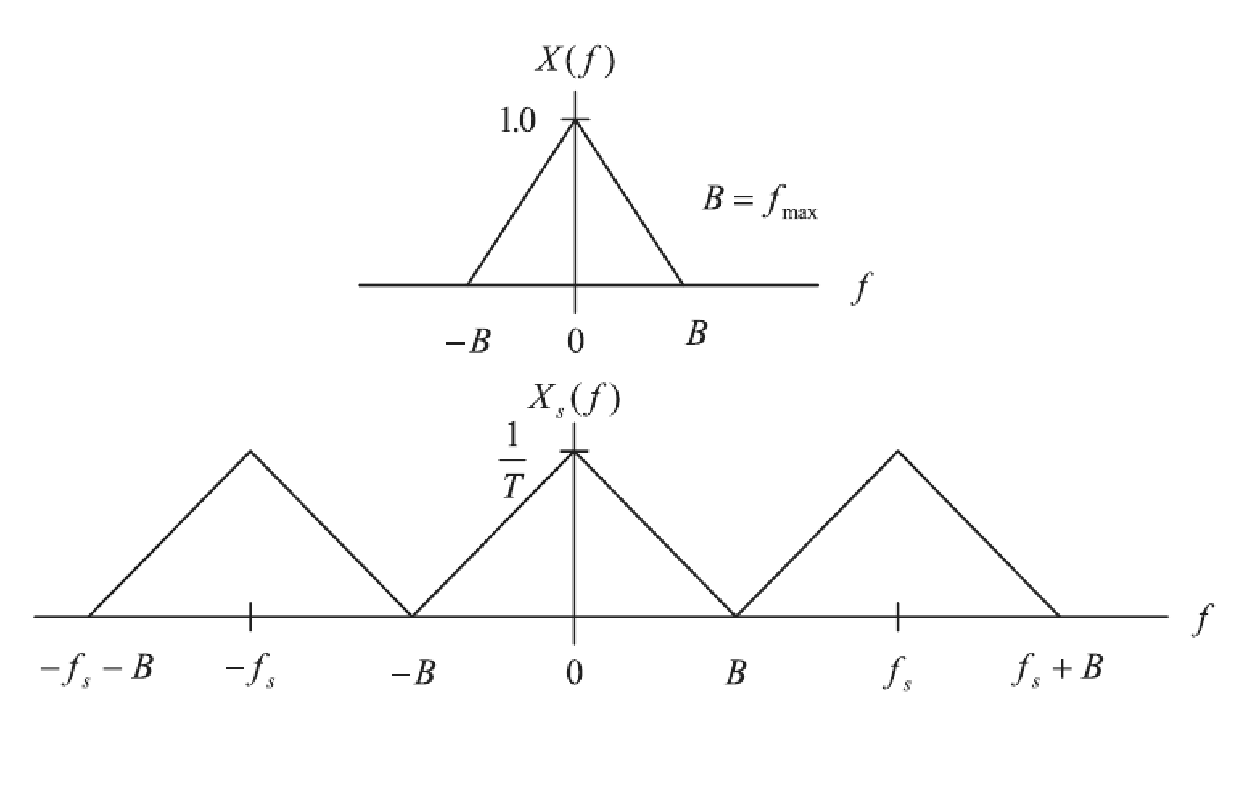
\includegraphics[width=0.9\linewidth]{./img/img10}
        \end{figure}
    \end{itemize}
\end{frame}

\begin{frame}{Teorema Sampling}
    \begin{itemize}
        \item Kondisi 3: spectrum sinyal sample overlapped dengan kembarannya
        \begin{figure}
            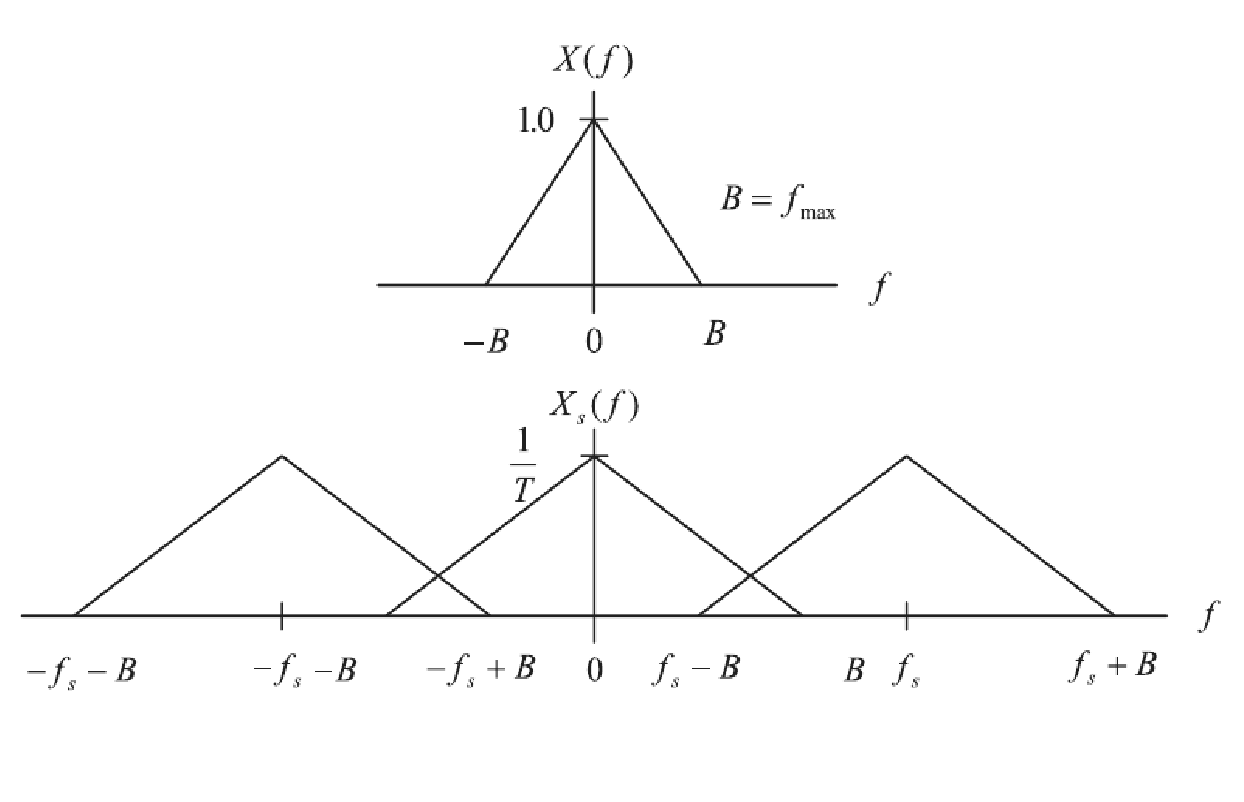
\includegraphics[width=0.9\linewidth]{./img/img11}
        \end{figure}
    \end{itemize}
\end{frame}

\begin{frame}{Teorema Sampling}
    \begin{itemize}
        \item Agar hasil rekonstruksi sinyal yang didapatkan nanti sama dengan sinyal analog yang asli, maka jangan sampai terjadi overlapped.
        \item Agar tidak terjadi overlapped, maka harus terpenuhi kondisi:
        \begin{equation}
            f_s - f_{\text{max}} \geq f_{\text{max}}
        \end{equation}
        dengan kata lain
        \begin{equation}
            f_s \geq 2f_{\text{max}}
            \label{eq:freq_nyquist}
        \end{equation}
        atau frekuensi dalam bentuk rad/sec.
        \begin{equation}
            \omega_s \geq 2\omega_{\text{max}}
        \end{equation}
        \item Teorema ini disebut sebagai \textbf{Shannon sampling theorem}
    \end{itemize} 
\end{frame}

\begin{frame}{Teorema Sampling}
    \begin{theorem}{\textbf{Shannon sampling theorem:}}
        For a uniformly sampled DSP system, an analog signal can be perfectly recovered as long as the sampling rate is at least twice as large as the highest-frequency component of the analog signal to be sampled.
    \end{theorem}
\end{frame}

\begin{frame}{Teorema Sampling}
    \begin{itemize}
        \item Karena sampling rate minimum sebesar 2 kali frekuensi maksimum dari sinyal analog. Dengan kata lain, frekuensi maksimum dari sinyal analog haruslah sama atau kurang dari setengah kali sampling rate-nya
        \begin{align*}
            f_s &\geq 2 f_\text{max} \\
            \frac{f_s}{2} &\geq f_\text{max}
        \end{align*}
        \item $\frac{f_s}{2}$ ini disebut sebagai frekuensi Nyquist
    \end{itemize}
\end{frame}

\begin{frame}{Contoh Soal 1}
    \begin{enumerate}
        \item Diketahui sinyal analog
        \begin{equation*}
            x(t) = 5 \cos (2 \pi 1000 t),~\text{ untuk } t \geq 0
        \end{equation*}
        dan sampling rate sebesar 8 kHz.
        \begin{enumerate}
            \item[a.] Gambarkan spectrum sinyal analog, $X(f)$
            \item[b.] Gambarkan spectrum sinyal sample, $X_s(f)$
        \end{enumerate}
    \end{enumerate}
\end{frame}

\begin{frame}{Jawaban Contoh Soal 1}
    \begin{itemize}
        \item Sinyal analog dapat kita tulis dalam bentuk Euler dengan menggunakan Pers. Euler
    \end{itemize}
    \begin{framed}
    \textbf{Pers. Euler}
        \begin{align}
            \sin(x) = \frac{(e^{jx} - e^{-jx})}{2j} \\
            \cos(x) = \frac{(e^{jx} + e^{-jx})}{2}
        \end{align}
    \end{framed}
\end{frame}

\begin{frame}{Jawaban Contoh Soal 1}
    \begin{itemize}
        \item sehingga
        \begin{align}
            x(t) &= 5 \cos (2 \pi 1000 t) = 5 \left( \frac{(e^{j2\pi 1000t} + e^{-j2\pi 1000t})}{2} \right) \\
            &= 2.5 e^{j2 \pi 1000t} + 2.5 e^{-j2 \pi 1000t}
            \label{eq:lat.soal.1}
        \end{align}
        \item Pers. (\ref{eq:lat.soal.1}) adalah bentuk complex-exponential dari deret Fourier.
        \item Bentuk umum dari complex-exponential dari deret Fourier:
        \begin{framed}
            \begin{equation*}
                x(t) = \sum_{k=-\infty}^{-\infty} c_k e^{jk\omega_0 t} = \sum_{k=-\infty}^{-\infty} c_k e^{jk 2\pi f_0 t}
            \end{equation*}
        \end{framed}
    \end{itemize}
\end{frame}

\begin{frame}{Jawaban Contoh Soal 1}
    \begin{itemize}
        \item Sehingga gambar spectrum sinyal analog, $X(f)$, adalah:
        \begin{figure}
            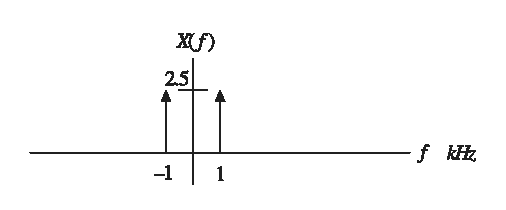
\includegraphics[width=\linewidth]{./img/img12}
        \end{figure}
    \end{itemize}
\end{frame}

\begin{frame}{Jawaban Contoh Soal 1}
    \begin{itemize}
        \item setelah analog signal di sampling dengan sampling rate 8000 Hz, maka spectrum sinyal sample dan kembarannya berada di frekuensi $\pm kf_s$ yang dengan scaled-amplitude sebesar $2.5/T$
        \begin{figure}
            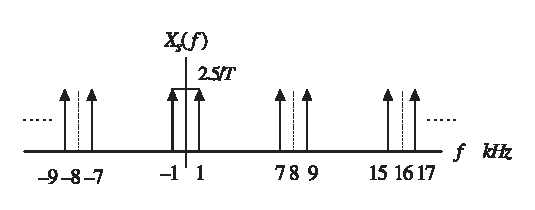
\includegraphics[width=\linewidth]{./img/img13}
        \end{figure}
    \end{itemize}
\end{frame}

\begin{frame}{Contoh Soal 2}
    \begin{enumerate}
        \setcounter{enumi}{1}
        \item Diketahui analog signal
        \begin{equation*}
            x(t) = 5 \cos (2 \pi 1500 t),~\text{ untuk } t \geq 0
        \end{equation*}
        dan sampling rate sebesar 8 kHz.
        \begin{enumerate}
            \item[a.] Gambarkan spectrum sinyal analog, $X(f)$
            \item[b.] Gambarkan spectrum sinyal sample, $X_s(f)$
        \end{enumerate}
    \end{enumerate}
\end{frame}

\begin{frame}{Contoh Soal 3}
    \begin{enumerate}
        \setcounter{enumi}{2}
        \item Diketahui analog signal
        \begin{equation*}
            x(t) = 5 \cos (2 \pi 1500 t) + 2 \cos (2 \pi 2200 t),~\text{ untuk } t \geq 0
        \end{equation*}
        dan sampling rate sebesar 8 kHz.
        \begin{enumerate}
            \item[a.] Gambarkan spectrum sinyal analog, $X(f)$
            \item[b.] Gambarkan spectrum sinyal sample, $X_s(f)$
        \end{enumerate}
    \end{enumerate}
\end{frame}

\begin{frame}{Contoh Soal 4}
    \begin{enumerate}
        \setcounter{enumi}{3}
        \item Diketahui analog signal
        \begin{equation*}
            x(t) = 3 \cos (2 \pi 2500 t) + 2 \cos (2 \pi 4200 t),~\text{ untuk } t \geq 0
        \end{equation*}
        dan sampling rate sebesar 8 kHz.
        \begin{enumerate}
            \item[a.] Gambarkan spectrum sinyal analog, $X(f)$
            \item[b.] Gambarkan spectrum sinyal sample, $X_s(f)$
        \end{enumerate}
    \end{enumerate}
\end{frame}

\section{Rekonstruksi Sinyal}

\begin{frame}{Rekonstruksi sinyal}
    \begin{figure}
        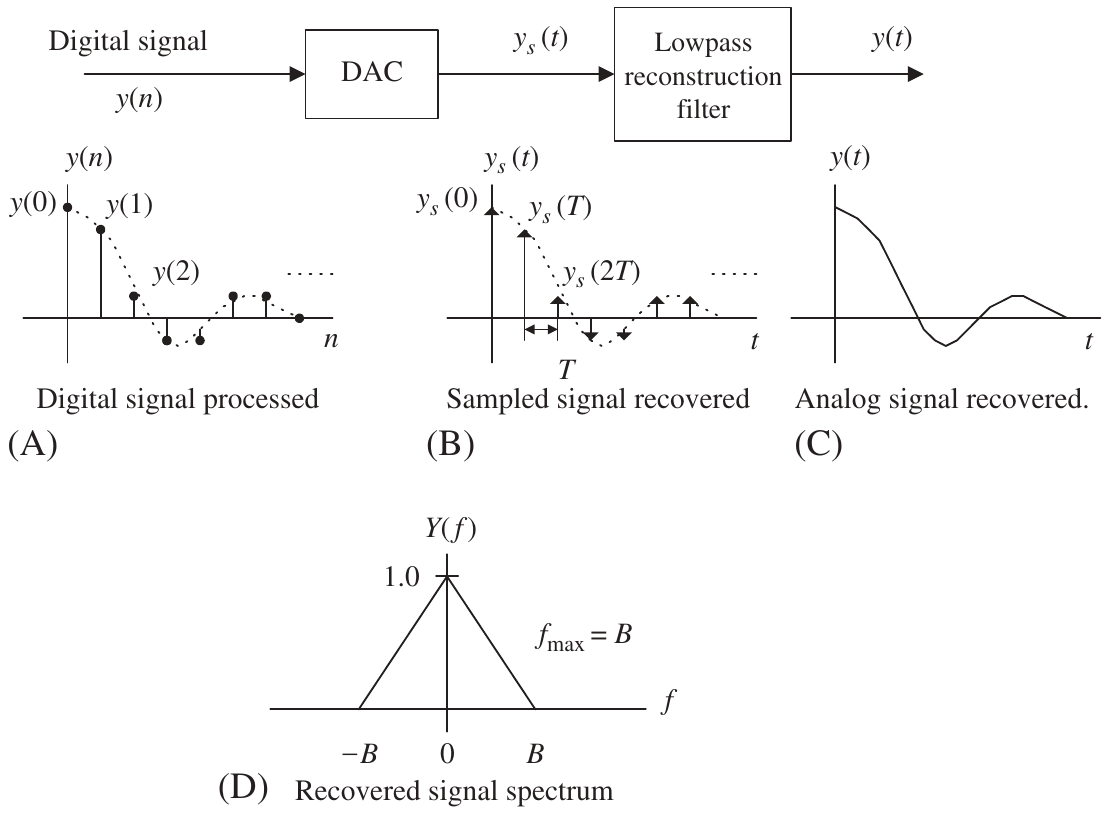
\includegraphics[width=0.9\linewidth]{img/img14.png}
    \end{figure}
\end{frame}

\begin{frame}{Rekonstruksi sinyal}
    \begin{enumerate}
        \item Kondisi 1: $f_s = 2f_{max}$
        \begin{itemize}
            \item Dibutuhkan ideal lowpass reconstruction filter
        \end{itemize}
    \end{enumerate}
    \begin{figure}
        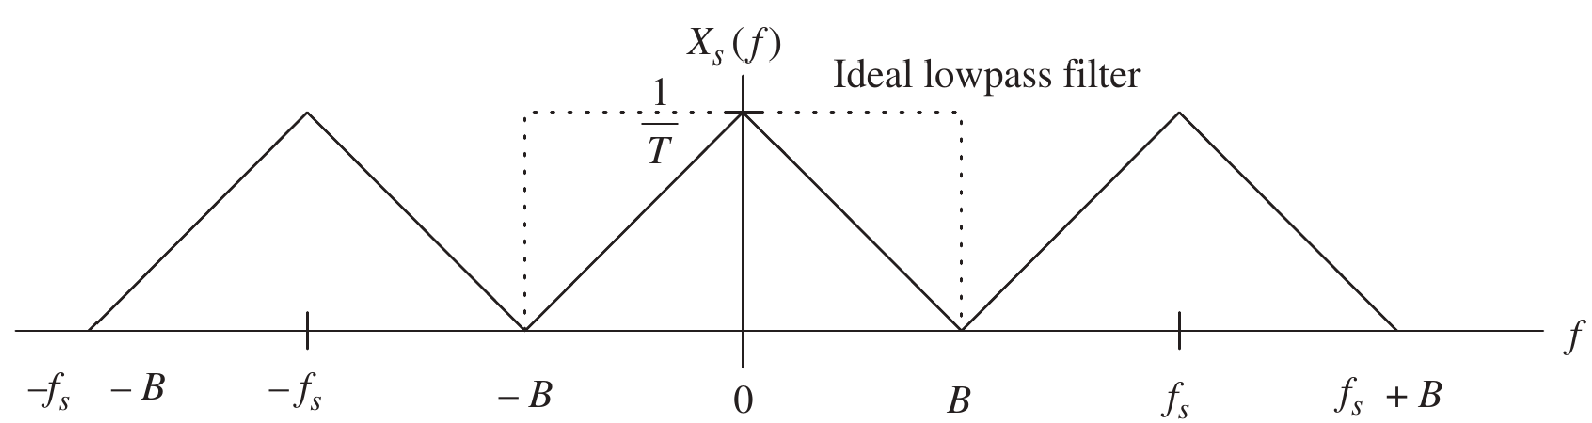
\includegraphics[width=\linewidth]{img/img15.png}
    \end{figure}
\end{frame}

\begin{frame}{Rekonstruksi sinyal}
    \begin{enumerate}
        \setcounter{enumi}{1}
        \item Kondisi 2: $f_s > 2f_{max}$
        \begin{itemize}
            \item Cukup practical lowpass reconstruction filter
        \end{itemize}
    \end{enumerate}
    \begin{figure}
        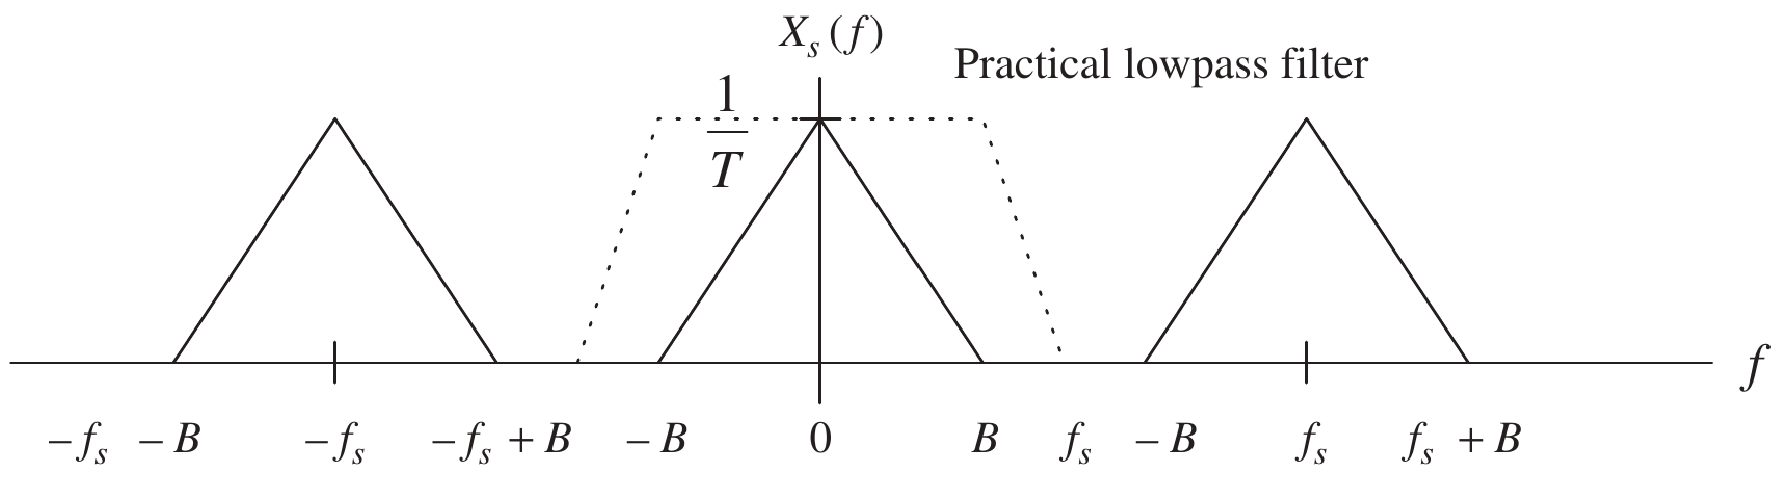
\includegraphics[width=\linewidth]{img/img16.png}
    \end{figure}
\end{frame}

\begin{frame}{Rekonstruksi sinyal}
    \begin{enumerate}
        \setcounter{enumi}{2}
        \item Kondisi 3: $f_s < 2f_{max}$
        \begin{itemize}
            \item Dibutuhkan ideal lowpass reconstruction filter
            \item Terdapat aliasing, menyebabkan distorsi spektral
            \item $f_\text{alias} = f_s - f$
        \end{itemize}
    \end{enumerate}
    \begin{figure}
        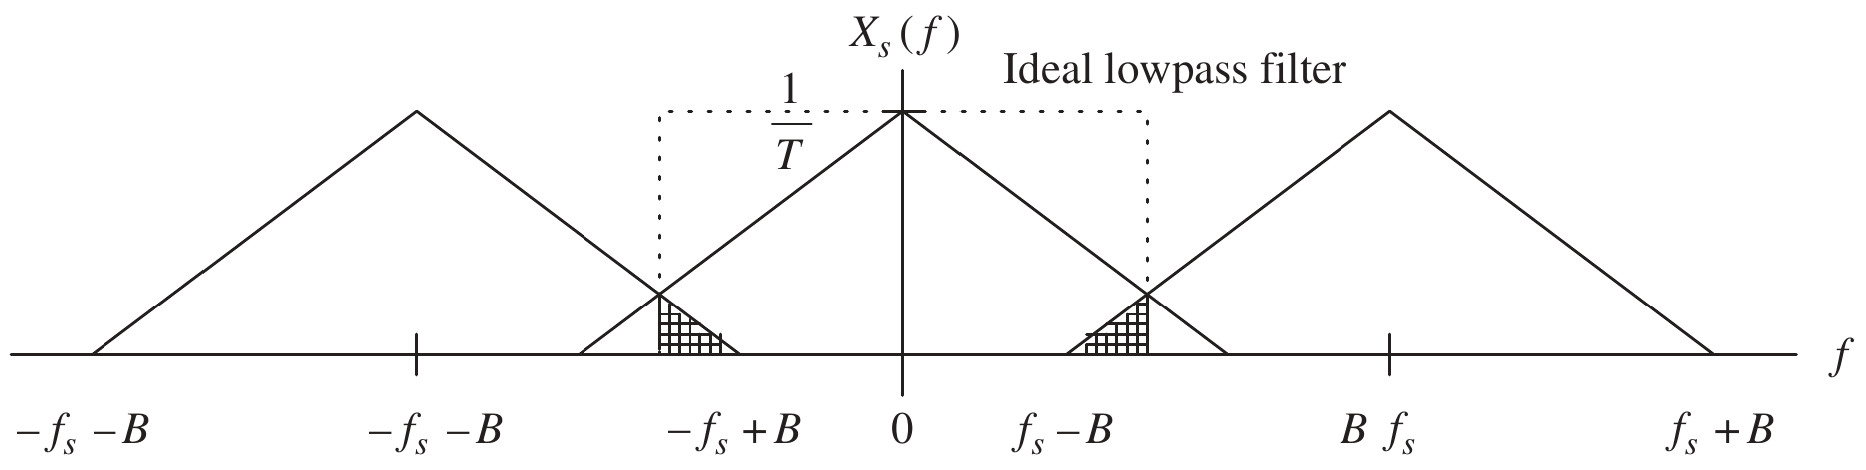
\includegraphics[width=\linewidth]{img/img17.png}
    \end{figure}
\end{frame}

\begin{frame}{Contoh Soal 5}
    Diasumsikan analog signal $$ x(t) = 5 \cos(2\pi 2000 t) + 3\cos(2\pi 3000t),~\text{ untuk } t \geq 0 $$ dengan sampling rate 8 kHz
    \begin{enumerate}
        \item[a)] Gambarkan spektrum sinyal sampled
        \item[b)] Gambarkan spektrum sinyal analog recovered jika ideal lowpass filter dengan cutoff-frequency 4 kHz.
    \end{enumerate}
\end{frame}

\begin{frame}{Jawaban Contoh Soal 5}
    \begin{enumerate}
        \item[a)] Menggunakan persamaan Euler
        $$x(t) = \frac{3}{2}e^{-j2 \pi 3000 t} + \frac{5}{2}e^{-j2 \pi 2000 t} + \frac{5}{2}e^{j2 \pi 2000 t} + \frac{3}{2}e^{j2 \pi 2000 t} $$
        Spektrum sinyal sampled
        \begin{figure}
            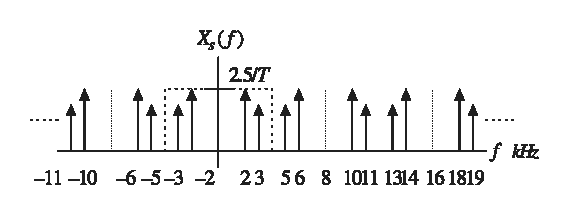
\includegraphics[width=\linewidth]{img/img18}
        \end{figure}
    \end{enumerate}
\end{frame}

\begin{frame}{Jawaban Contoh Soal 5}
    \begin{enumerate}
        \item[b)] Spektrum sinyal analog recovered tanpa ada noise dari aliasing.
        \begin{figure}
            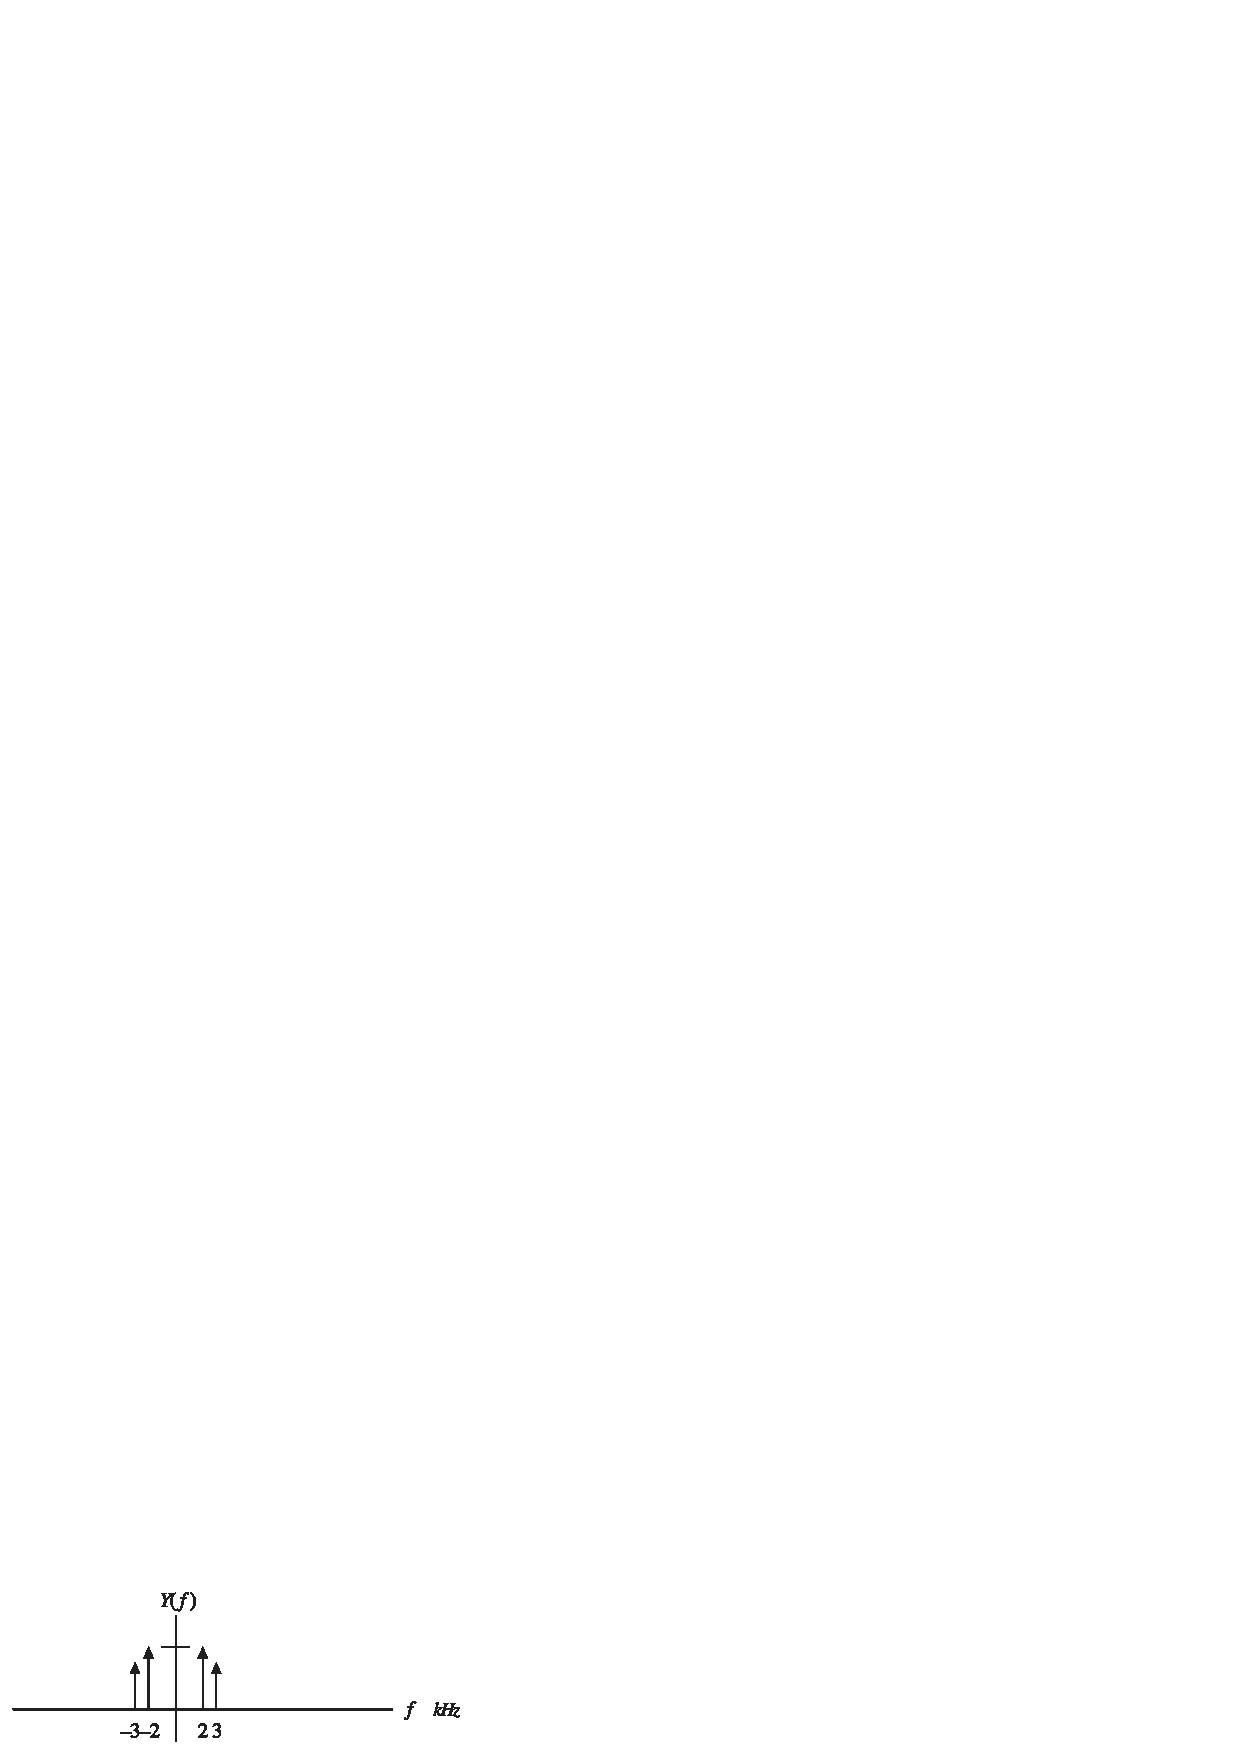
\includegraphics[width=\linewidth]{img/img19}
        \end{figure}
    \end{enumerate}
\end{frame}

\begin{frame}{Contoh Soal 6}
    Diasumsikan analog signal $$ x(t) = 5 \cos(2\pi 2000 t) + \cos(2\pi 5000t),~\text{ untuk } t \geq 0 $$ dengan sampling rate 8 kHz
    \begin{enumerate}
        \item[a)] Gambarkan spektrum sinyal sampled
        \item[b)] Gambarkan spektrum sinyal analog recovered jika ideal lowpass filter dengan cutoff-frequency 4 kHz.
    \end{enumerate}
\end{frame}

\begin{frame}{Jawaban Contoh Soal 6}
    \begin{enumerate}
        \item[a)] Menggunakan persamaan Euler
        $$x(t) = \frac{1}{2}e^{-j2 \pi 5000 t} + \frac{5}{2}e^{-j2 \pi 2000 t} + \frac{5}{2}e^{j2 \pi 2000 t} + \frac{1}{2}e^{j2 \pi 2000 t} $$
        Spektrum sinyal sampled
        \begin{figure}
            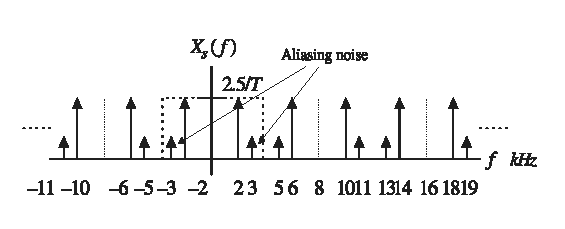
\includegraphics[width=\linewidth]{img/img20}
        \end{figure}
    \end{enumerate}
\end{frame}

\begin{frame}{Jawaban Contoh Soal 6}
    \begin{enumerate}
        \item[b)] Karena frekuensi maksimum dari sinyal analog lebih besar daripada frekuensi Nyquist-nya maka spektrum sinyal analog recovered memiliki aliasing noise di frekuensi 3 kHz:
        \begin{figure}
            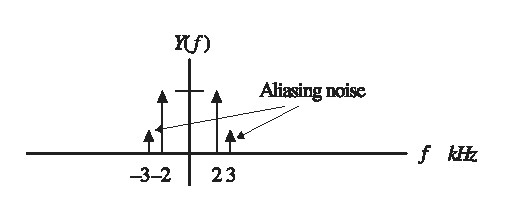
\includegraphics[width=\linewidth]{img/img21}
        \end{figure}
    \end{enumerate}
\end{frame}

\end{document}